\newpage
\chapter{Sensitivity Analysis} \label{ch:sensitivity}

The trade-off tool created to evaluate the concepts is quite complex and has many inter-dependencies. Each of these relations was plotted across a reasonable range of variance against all the significant outputs. Some of the most significant and interesting plots are discussed in this chapter. The trade-off criteria showed little sensitivity for many of the inputs and assumptions plotted. Those plots were either entirely independent of the input, or each of the concepts showed proportional effects, and will have little effect on the trade-off.

\section{Pad Costs}
It was determined that the pad cost could be a major driver of ticker 

pad costs drive ticket price

market \%








\begin{figure}[H]
\begin{subfigure}[t]{0.33\textwidth}
    \centering
    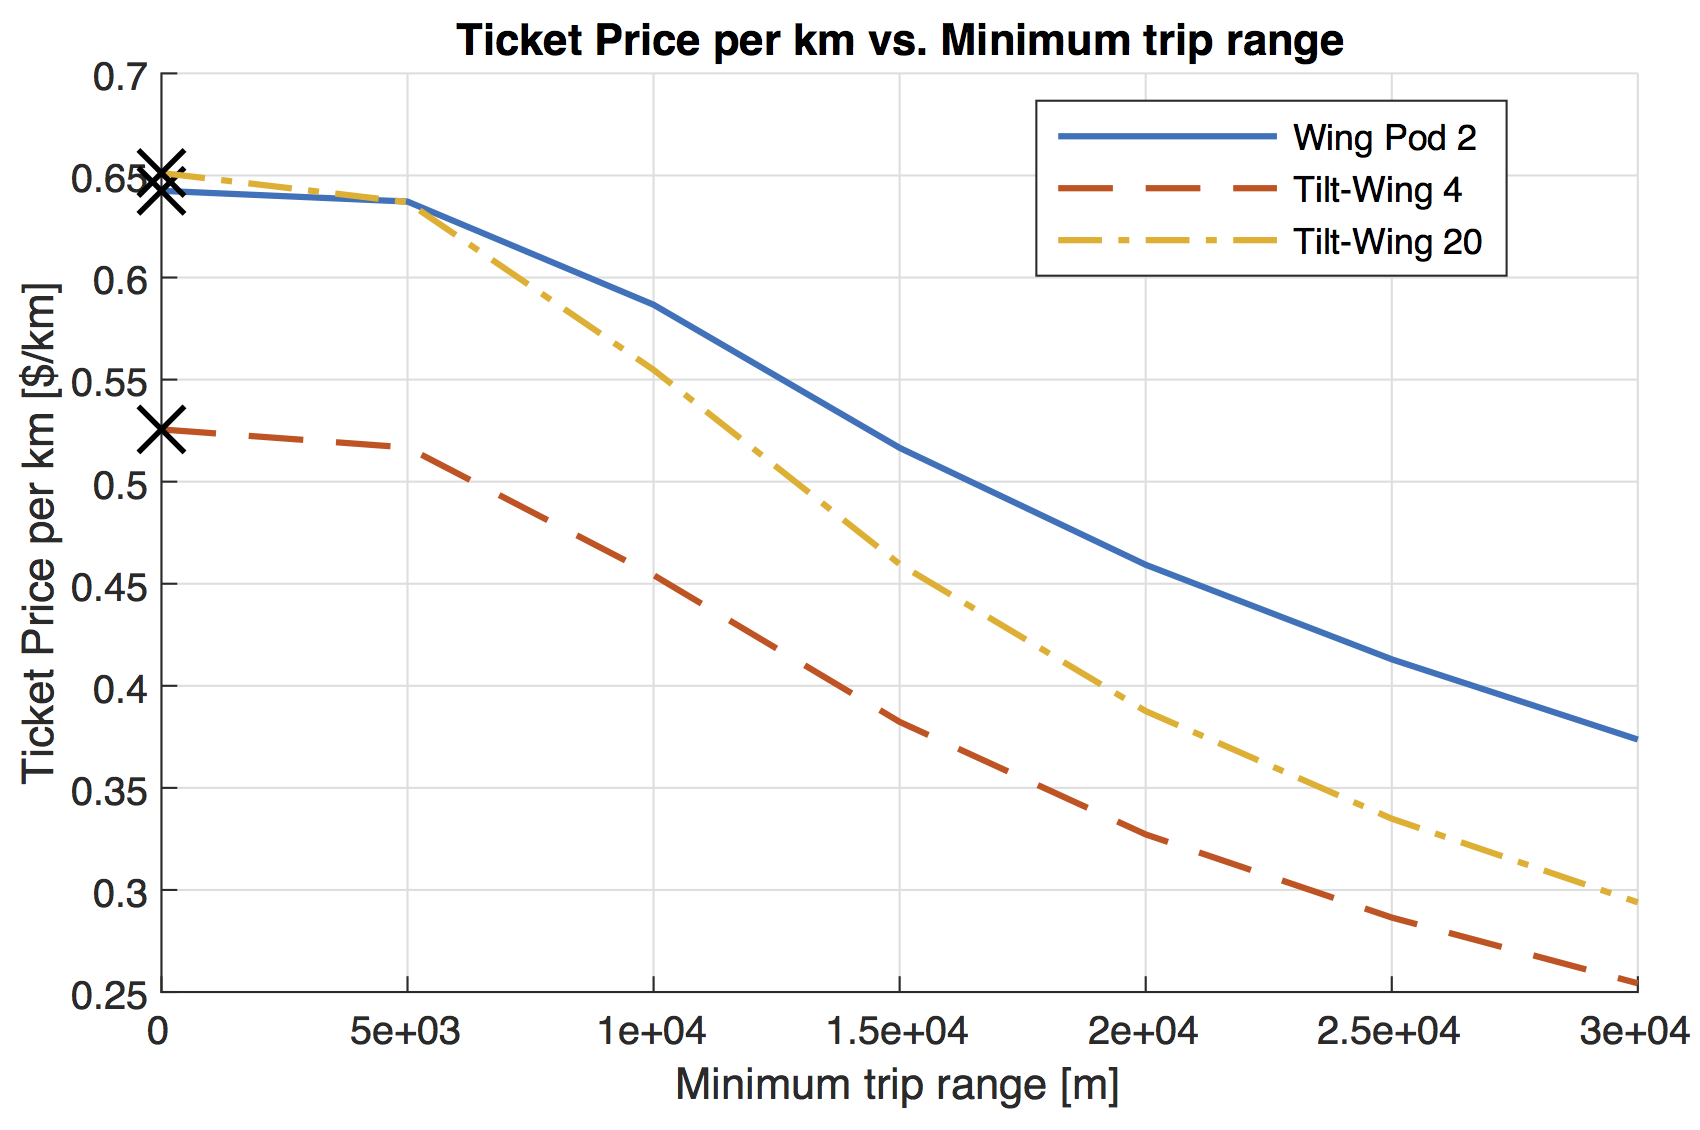
\includegraphics[width=\textwidth]{Figures/minRange_TPrice_perkmNOPAD.png}
    \captionsetup{justification=centering}
    \caption{OEW/MTOW}
    \label{fig:sens1}
\end{subfigure}
\begin{subfigure}[t]{0.33\textwidth}
    \centering
    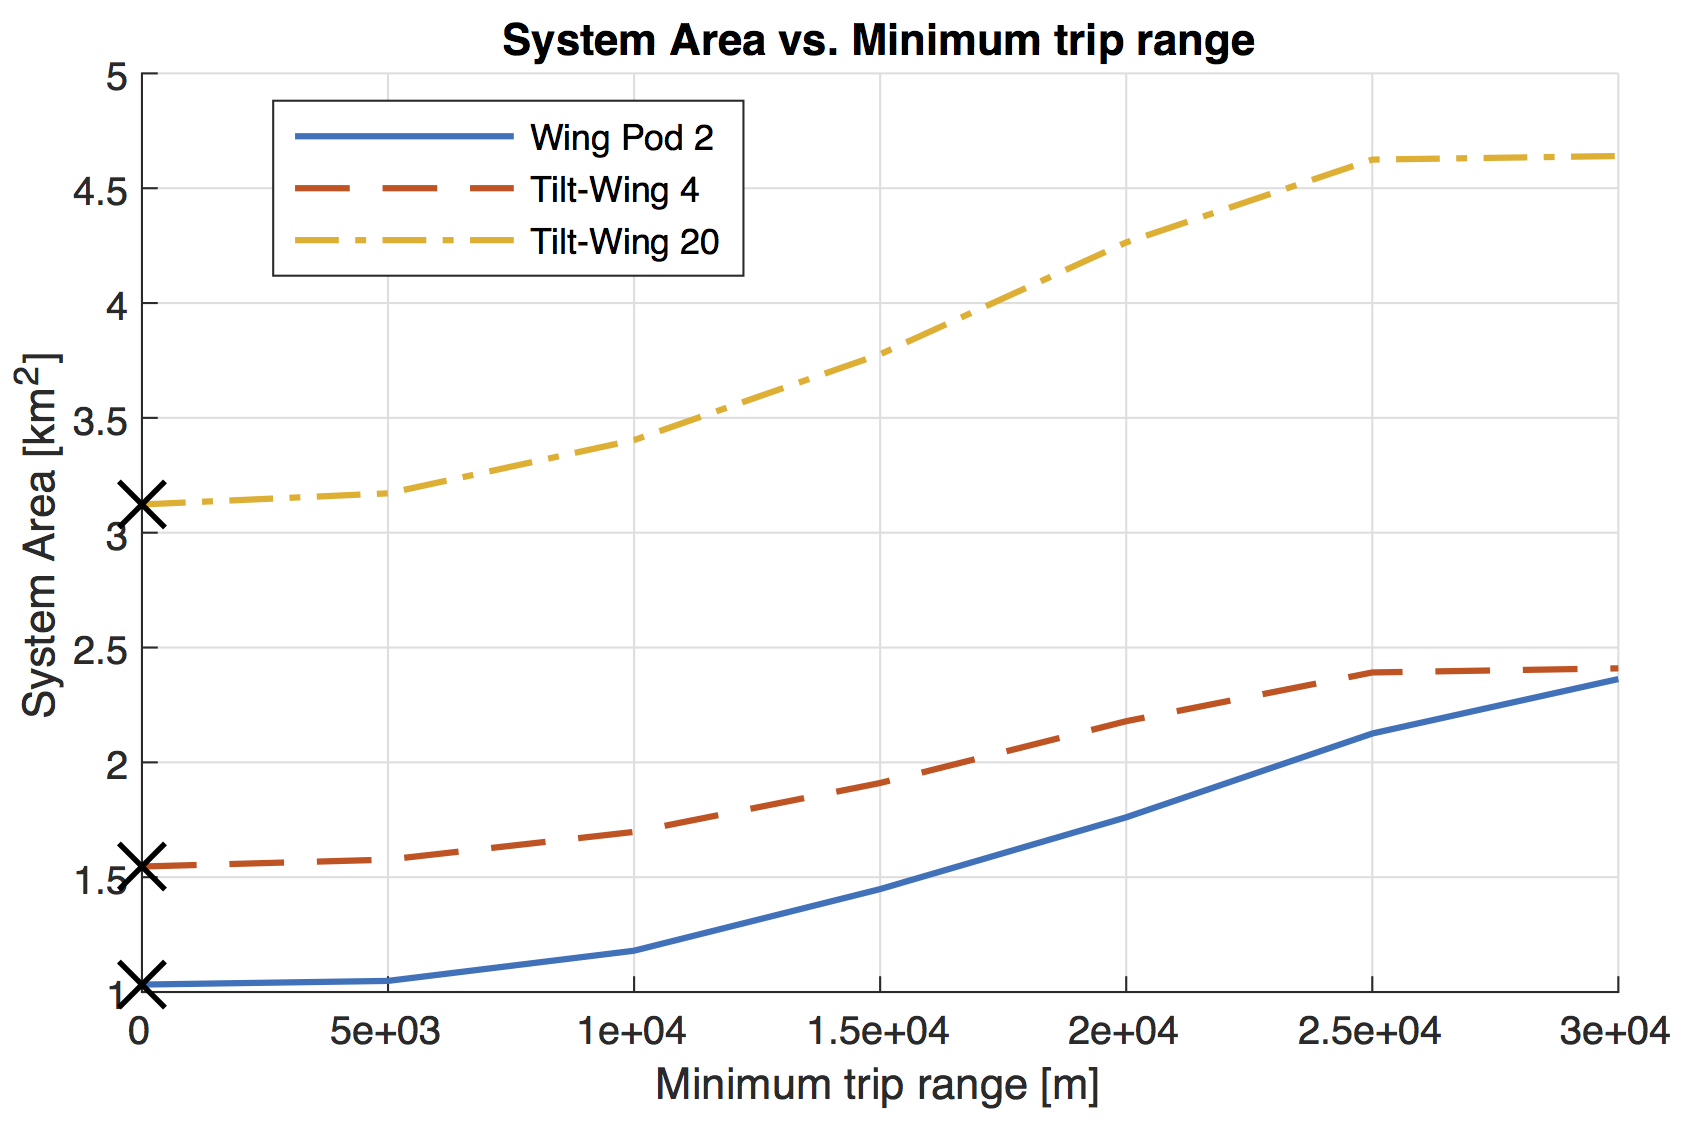
\includegraphics[width=\textwidth]{Figures/report_sys_area.png}
    \captionsetup{justification=centering}
    \caption{}
    \label{fig:sens2}
\end{subfigure}
\begin{subfigure}[t]{0.33\textwidth}
    \centering
    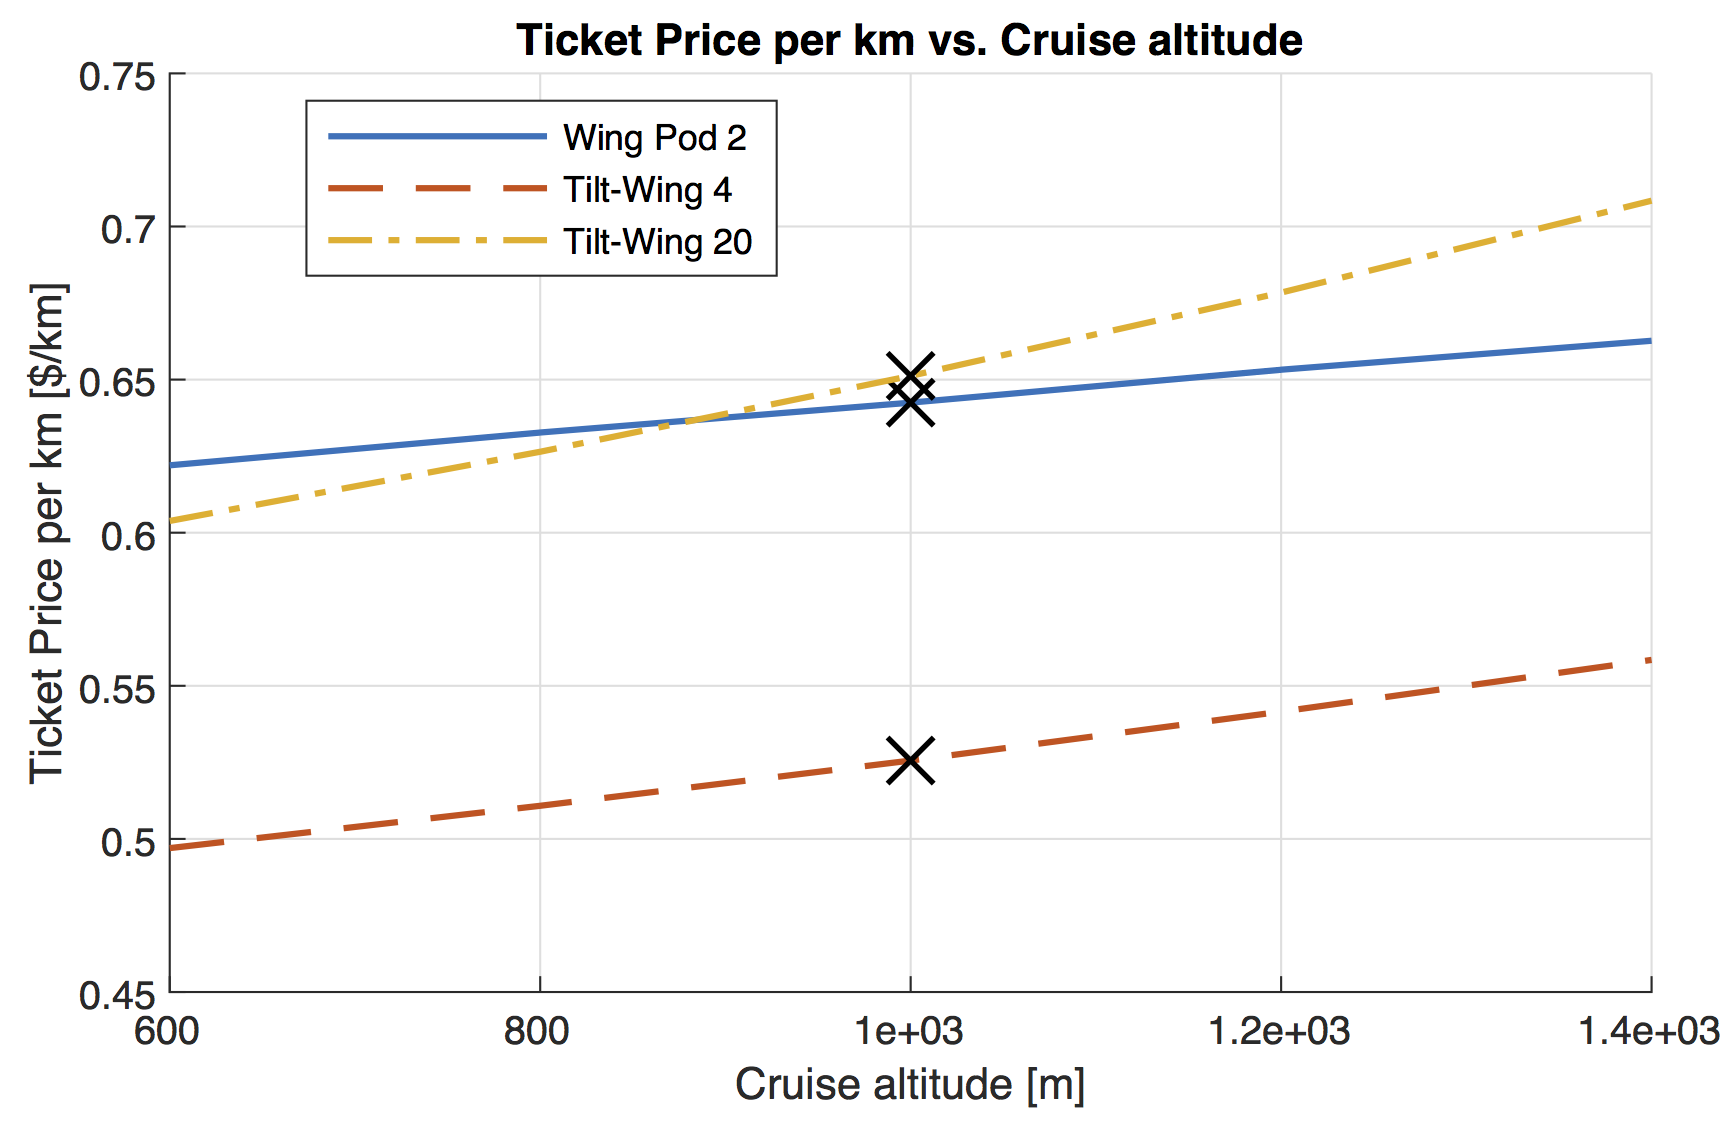
\includegraphics[width=\textwidth]{Figures/Alt_TPrice_perkmNOPAD.png}
    \captionsetup{justification=centering}
    \caption{}
    \label{fig:sens3}
\end{subfigure}
\captionsetup{justification=centering}
\caption{}
\label{fig:sens123}
\end{figure}




\begin{figure}[H]
\begin{subfigure}[t]{0.33\textwidth}
    \centering
    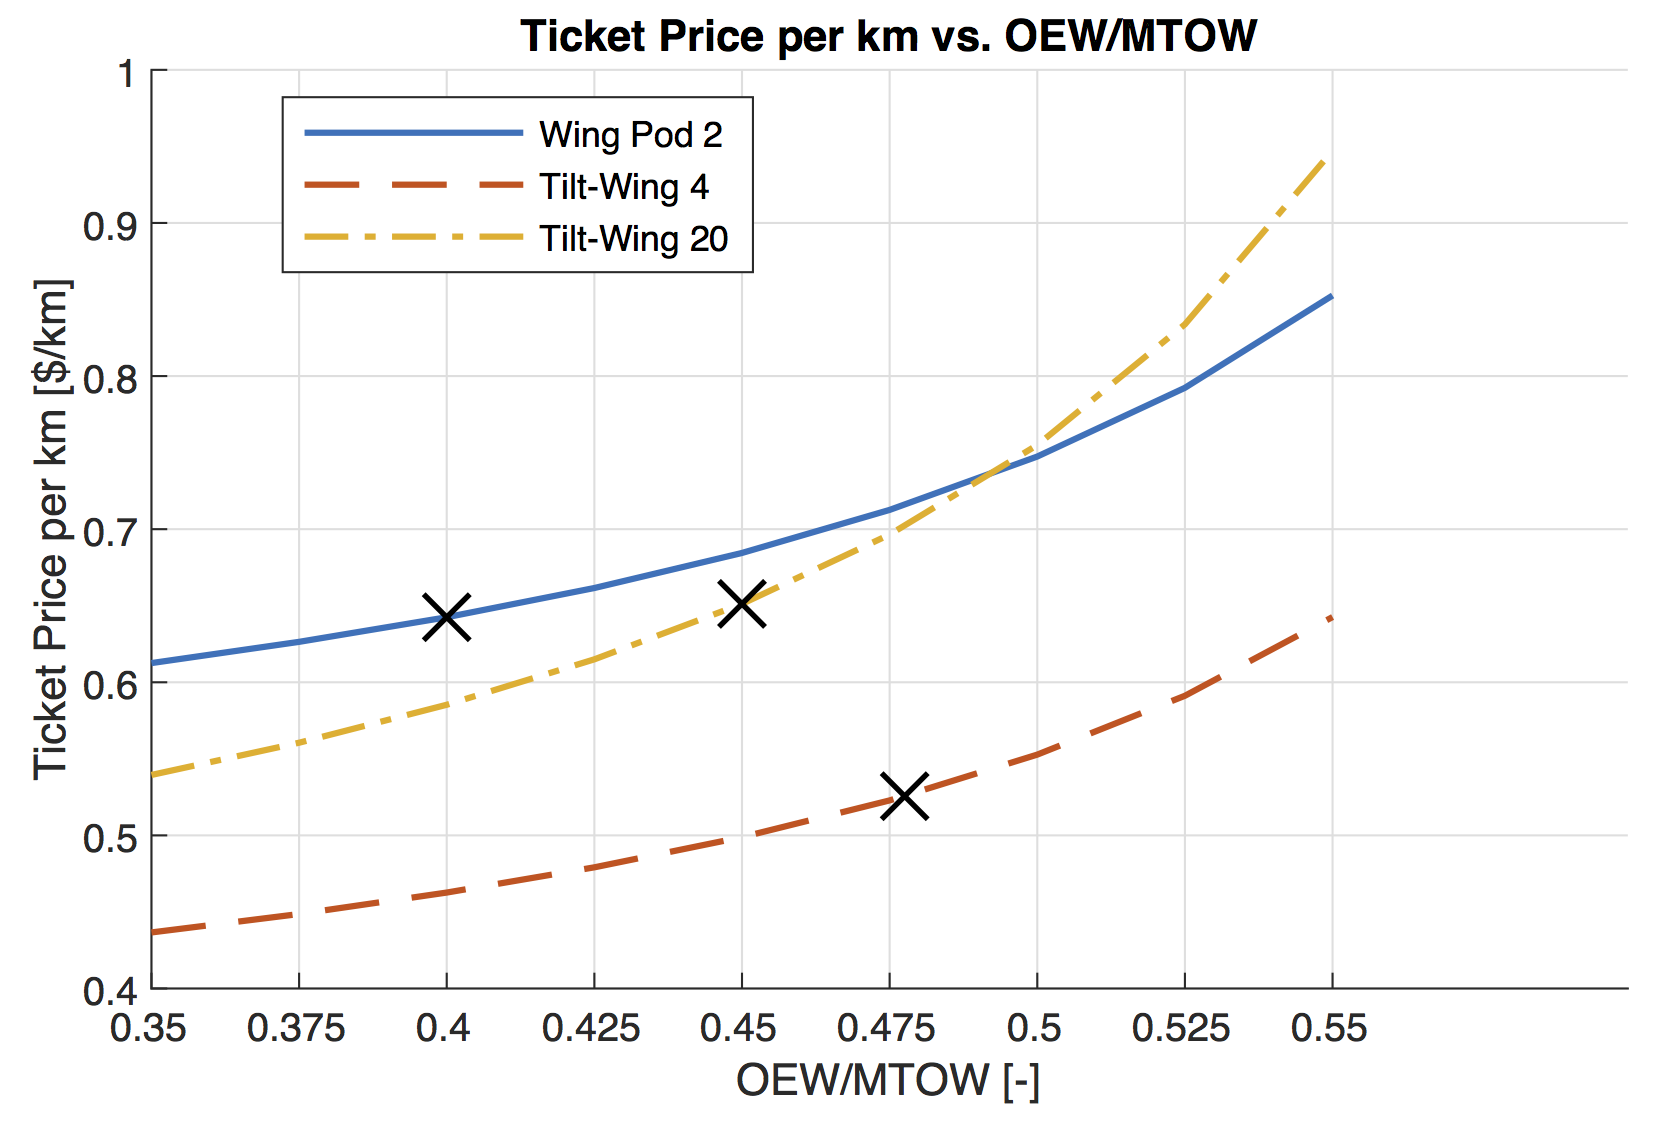
\includegraphics[width=\textwidth]{Figures/OEWMTOW_TPrice_perkmNOPAD.png}
    \captionsetup{justification=centering}
    \caption{OEW/MTOW}
    \label{fig:sens4}
\end{subfigure}
\begin{subfigure}[t]{0.33\textwidth}
    \centering
    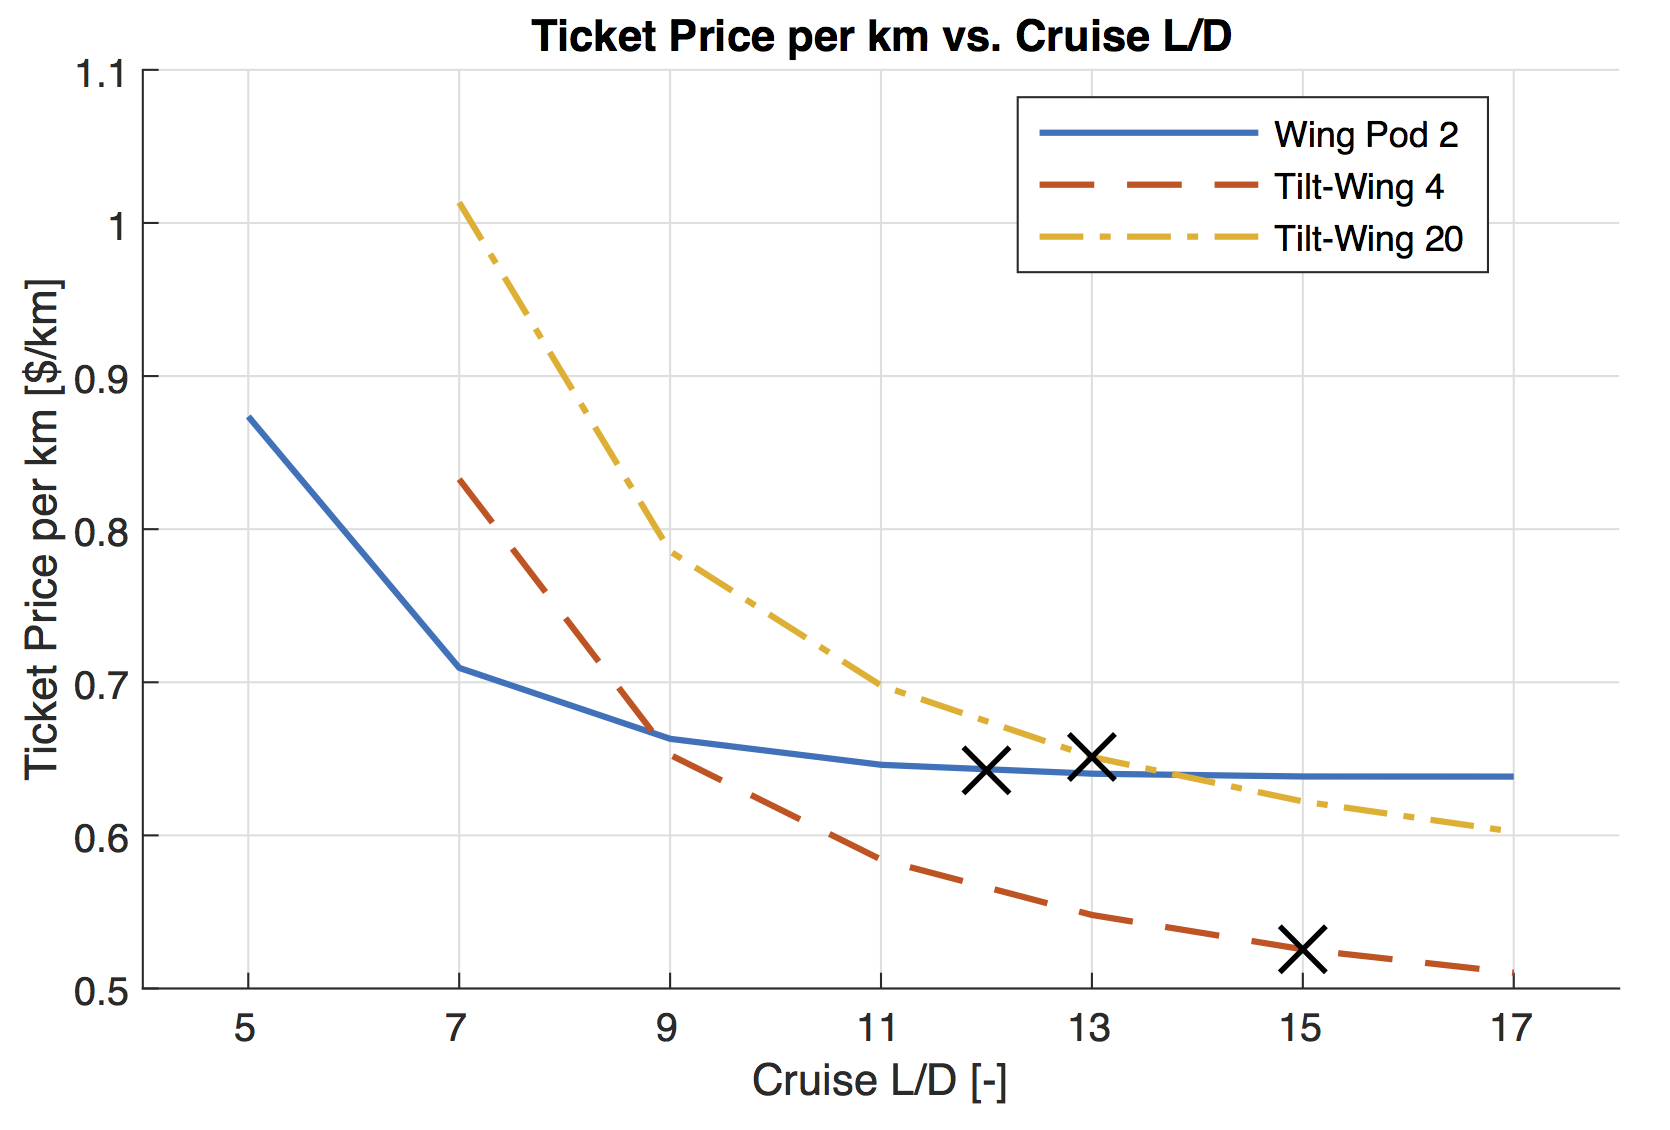
\includegraphics[width=\textwidth]{Figures/LoD_TPrice_perkmNOPAD.png}
    \captionsetup{justification=centering}
    \caption{}
    \label{fig:sens5}
\end{subfigure}
\begin{subfigure}[t]{0.33\textwidth}
    \centering
    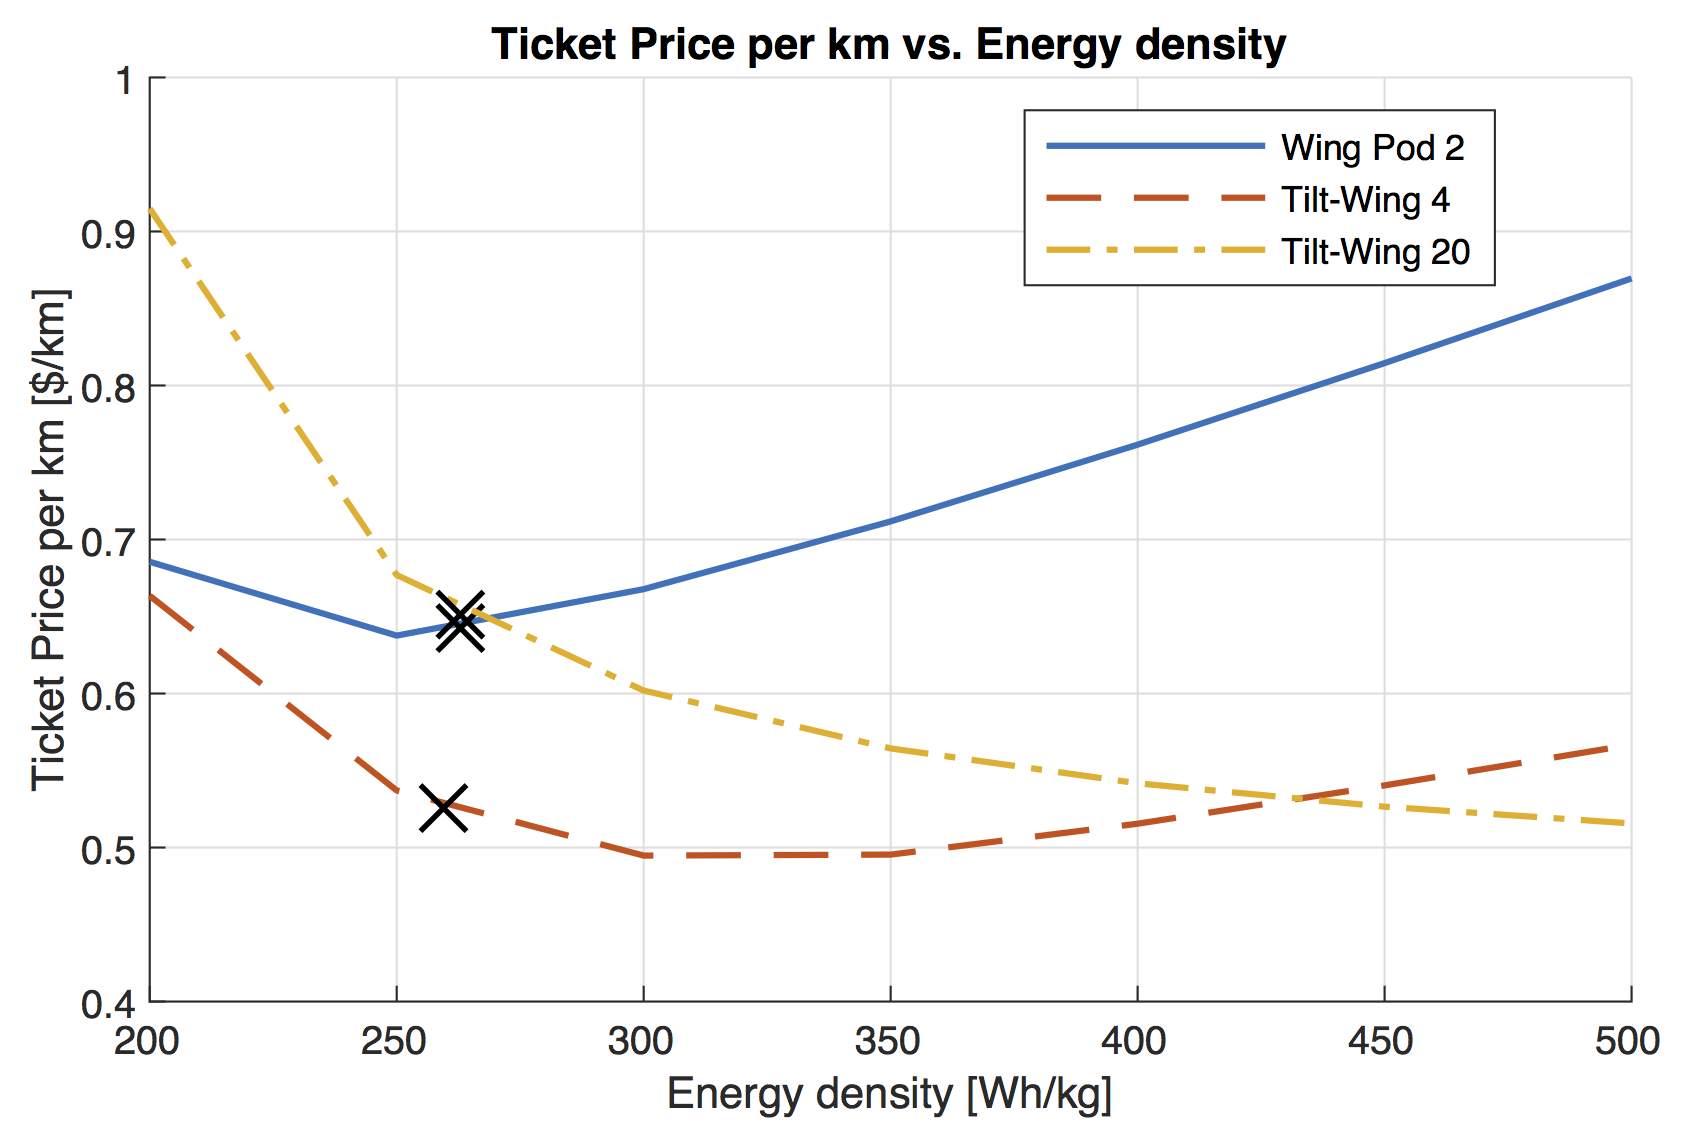
\includegraphics[width=\textwidth]{Figures/Edens_TPrice_perkmNOPAD.png}
    \captionsetup{justification=centering}
    \caption{}
    \label{fig:sens6}
\end{subfigure}
\captionsetup{justification=centering}
\caption{}
\label{fig:sens456}
\end{figure}

\begin{figure}[H]
\begin{subfigure}[t]{0.33\textwidth}
    \centering
    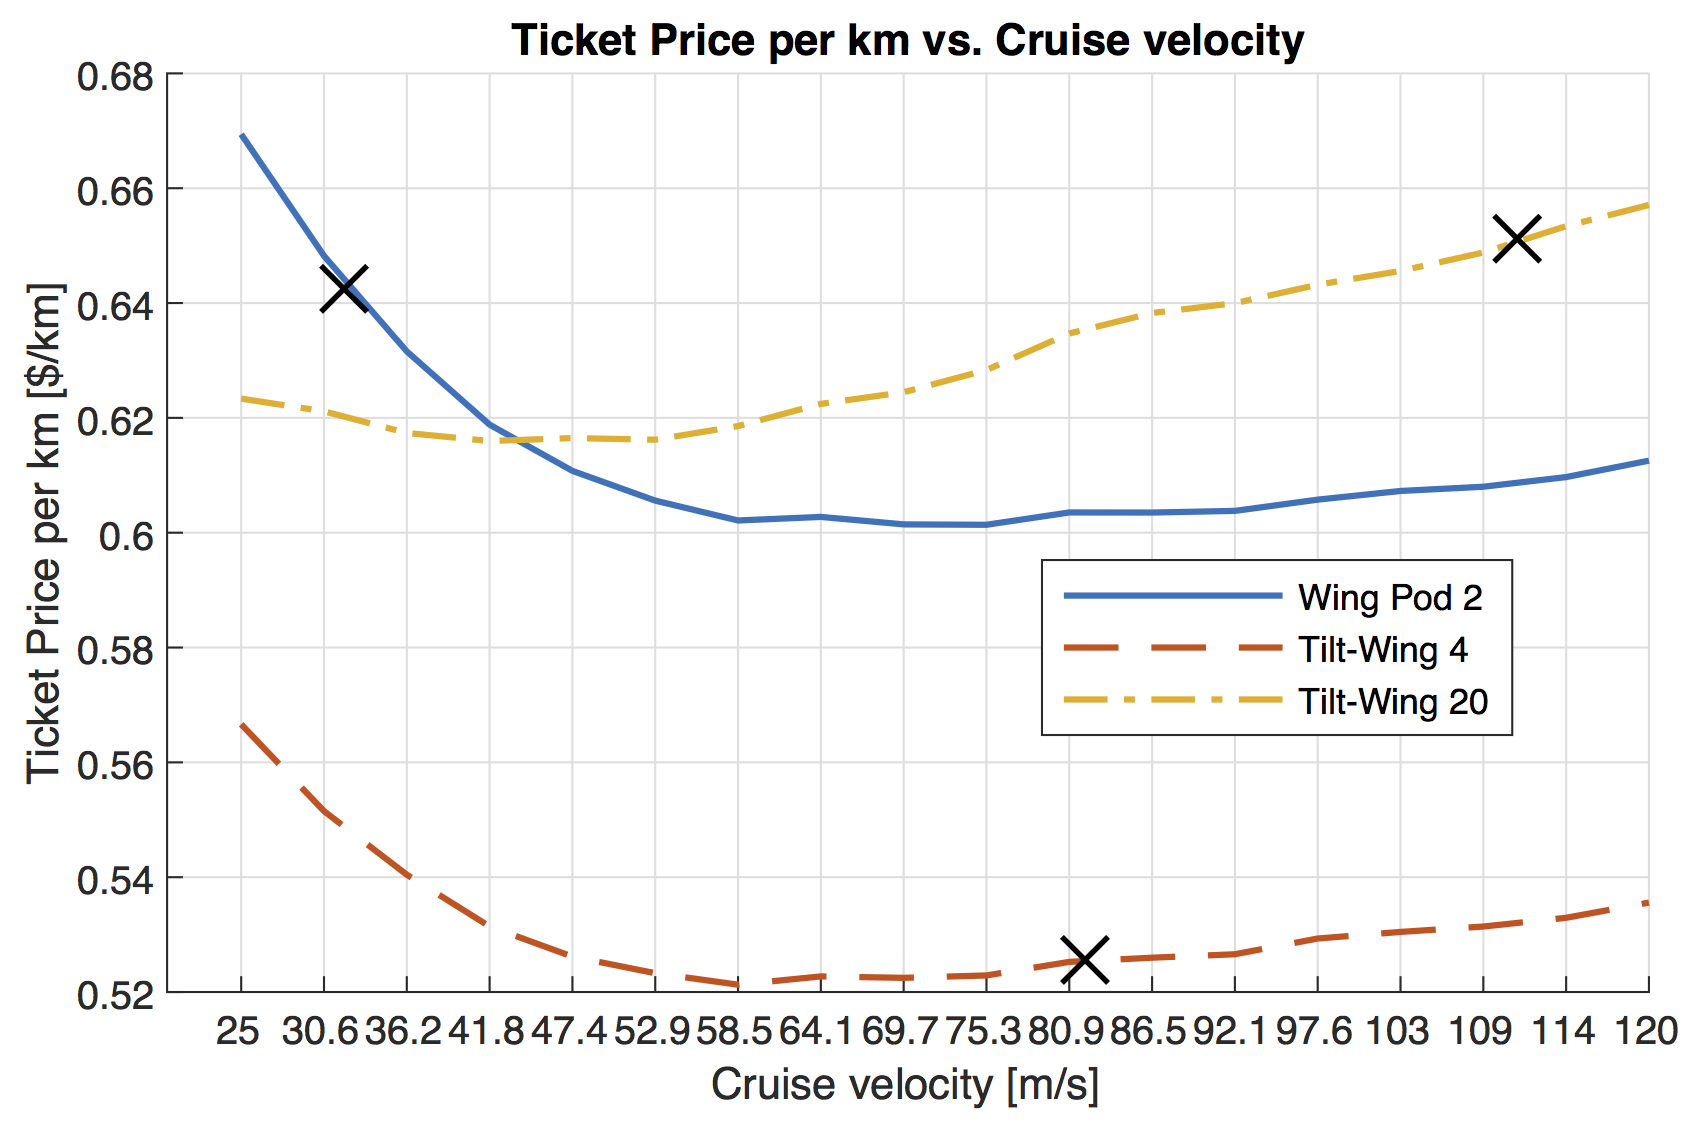
\includegraphics[width=\textwidth]{Figures/Cruise_TPrice_perkmNOPAD.png}
    \captionsetup{justification=centering}
    \caption{OEW/MTOW}
    \label{fig:sens7}
\end{subfigure}
\begin{subfigure}[t]{0.33\textwidth}
    \centering
    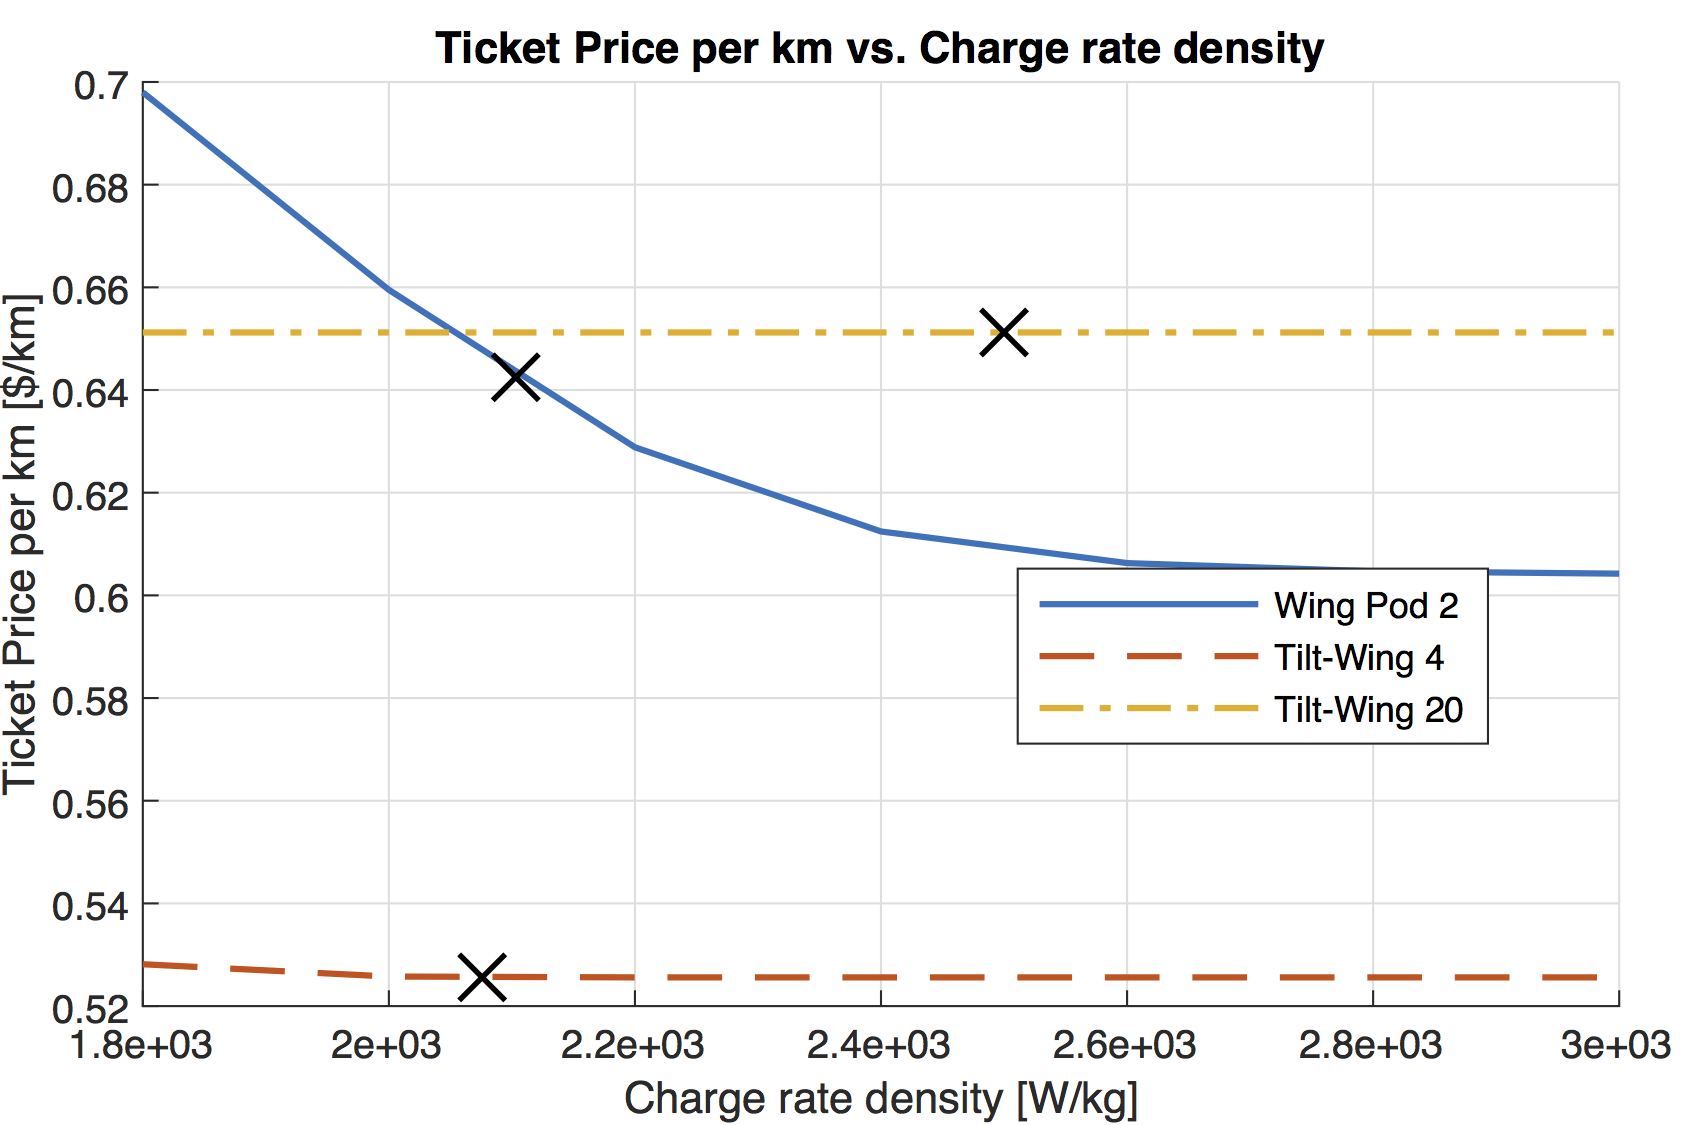
\includegraphics[width=\textwidth]{Figures/CRate_TPrice_perkmNOPAD.png}
    \captionsetup{justification=centering}
    \caption{}
    \label{fig:sens8}
\end{subfigure}
\begin{subfigure}[t]{0.33\textwidth}
    \centering
    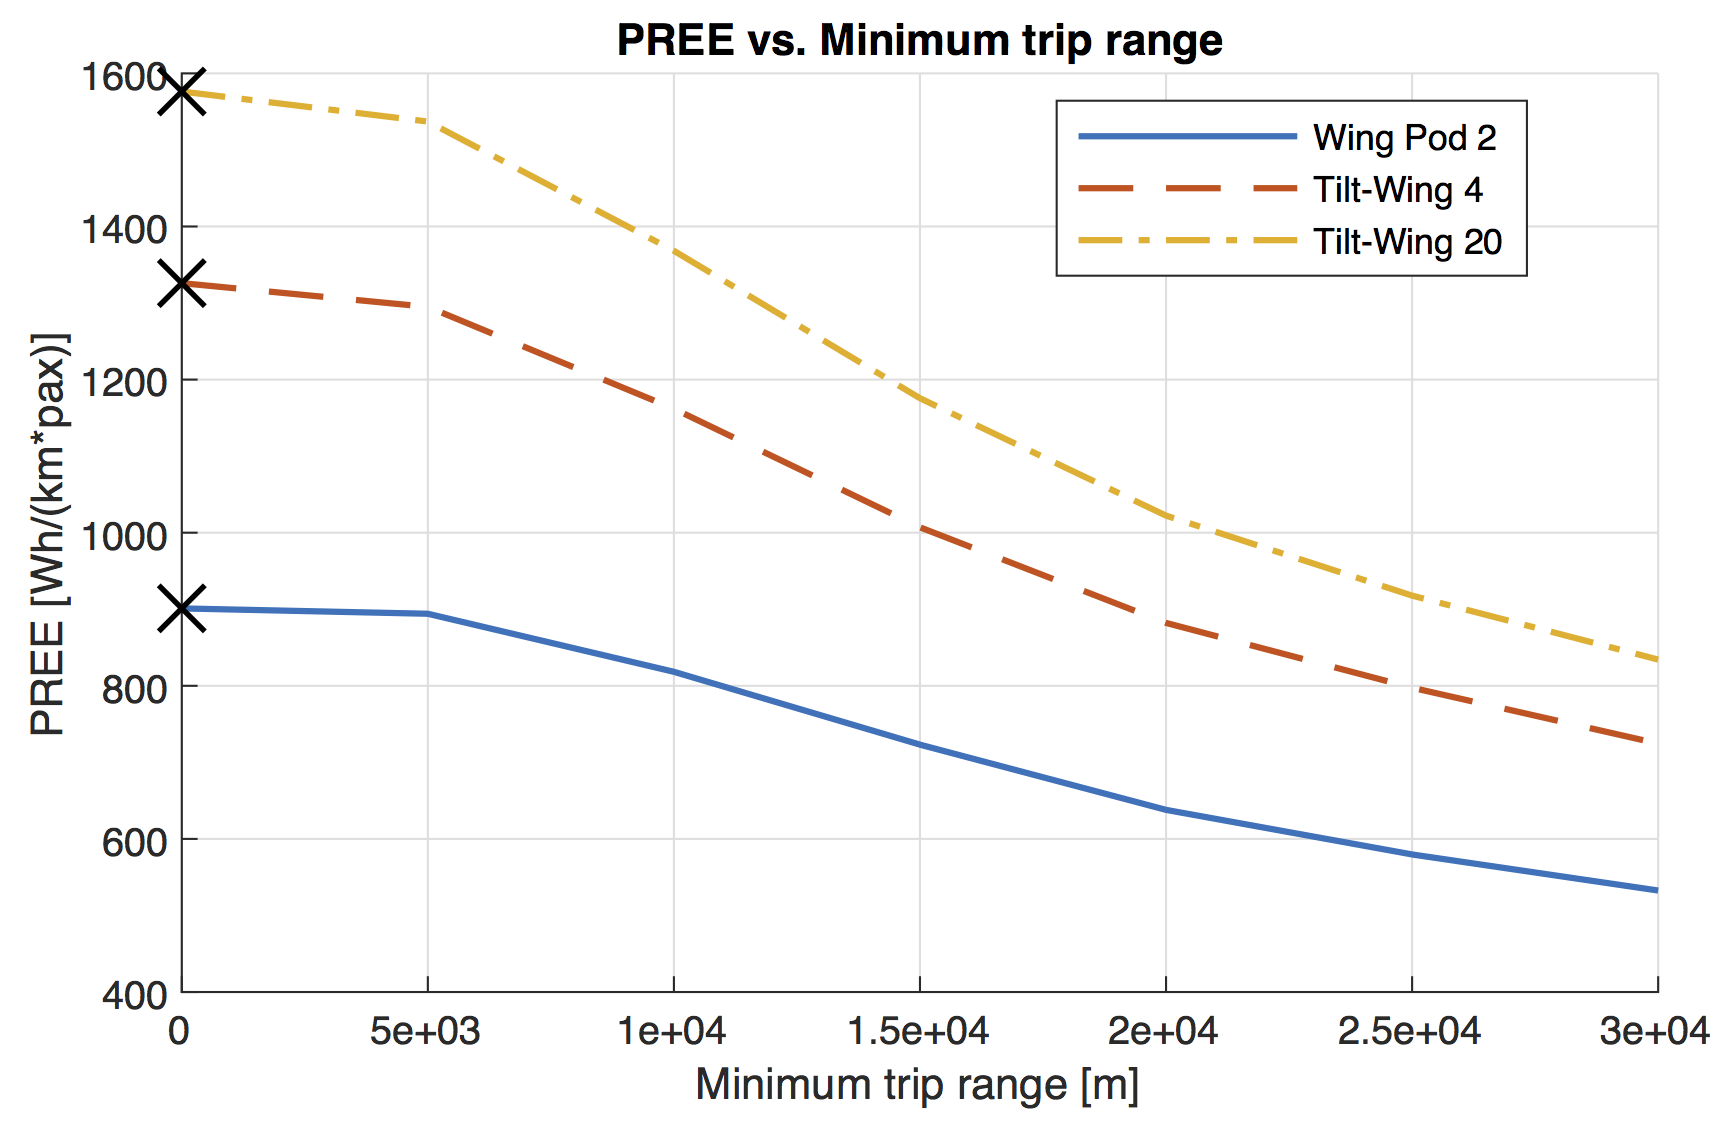
\includegraphics[width=\textwidth]{Figures/report_PREE.png}
    \captionsetup{justification=centering}
    \caption{}
    \label{fig:sens9}
\end{subfigure}
\captionsetup{justification=centering}
\caption{}
\label{fig:sens789}
\end{figure}

\subsection{Autonomous and Remotely Assisted Piloting}

\begin{wrapfigure}[18]{r}{0.35\textwidth}
    \centering
    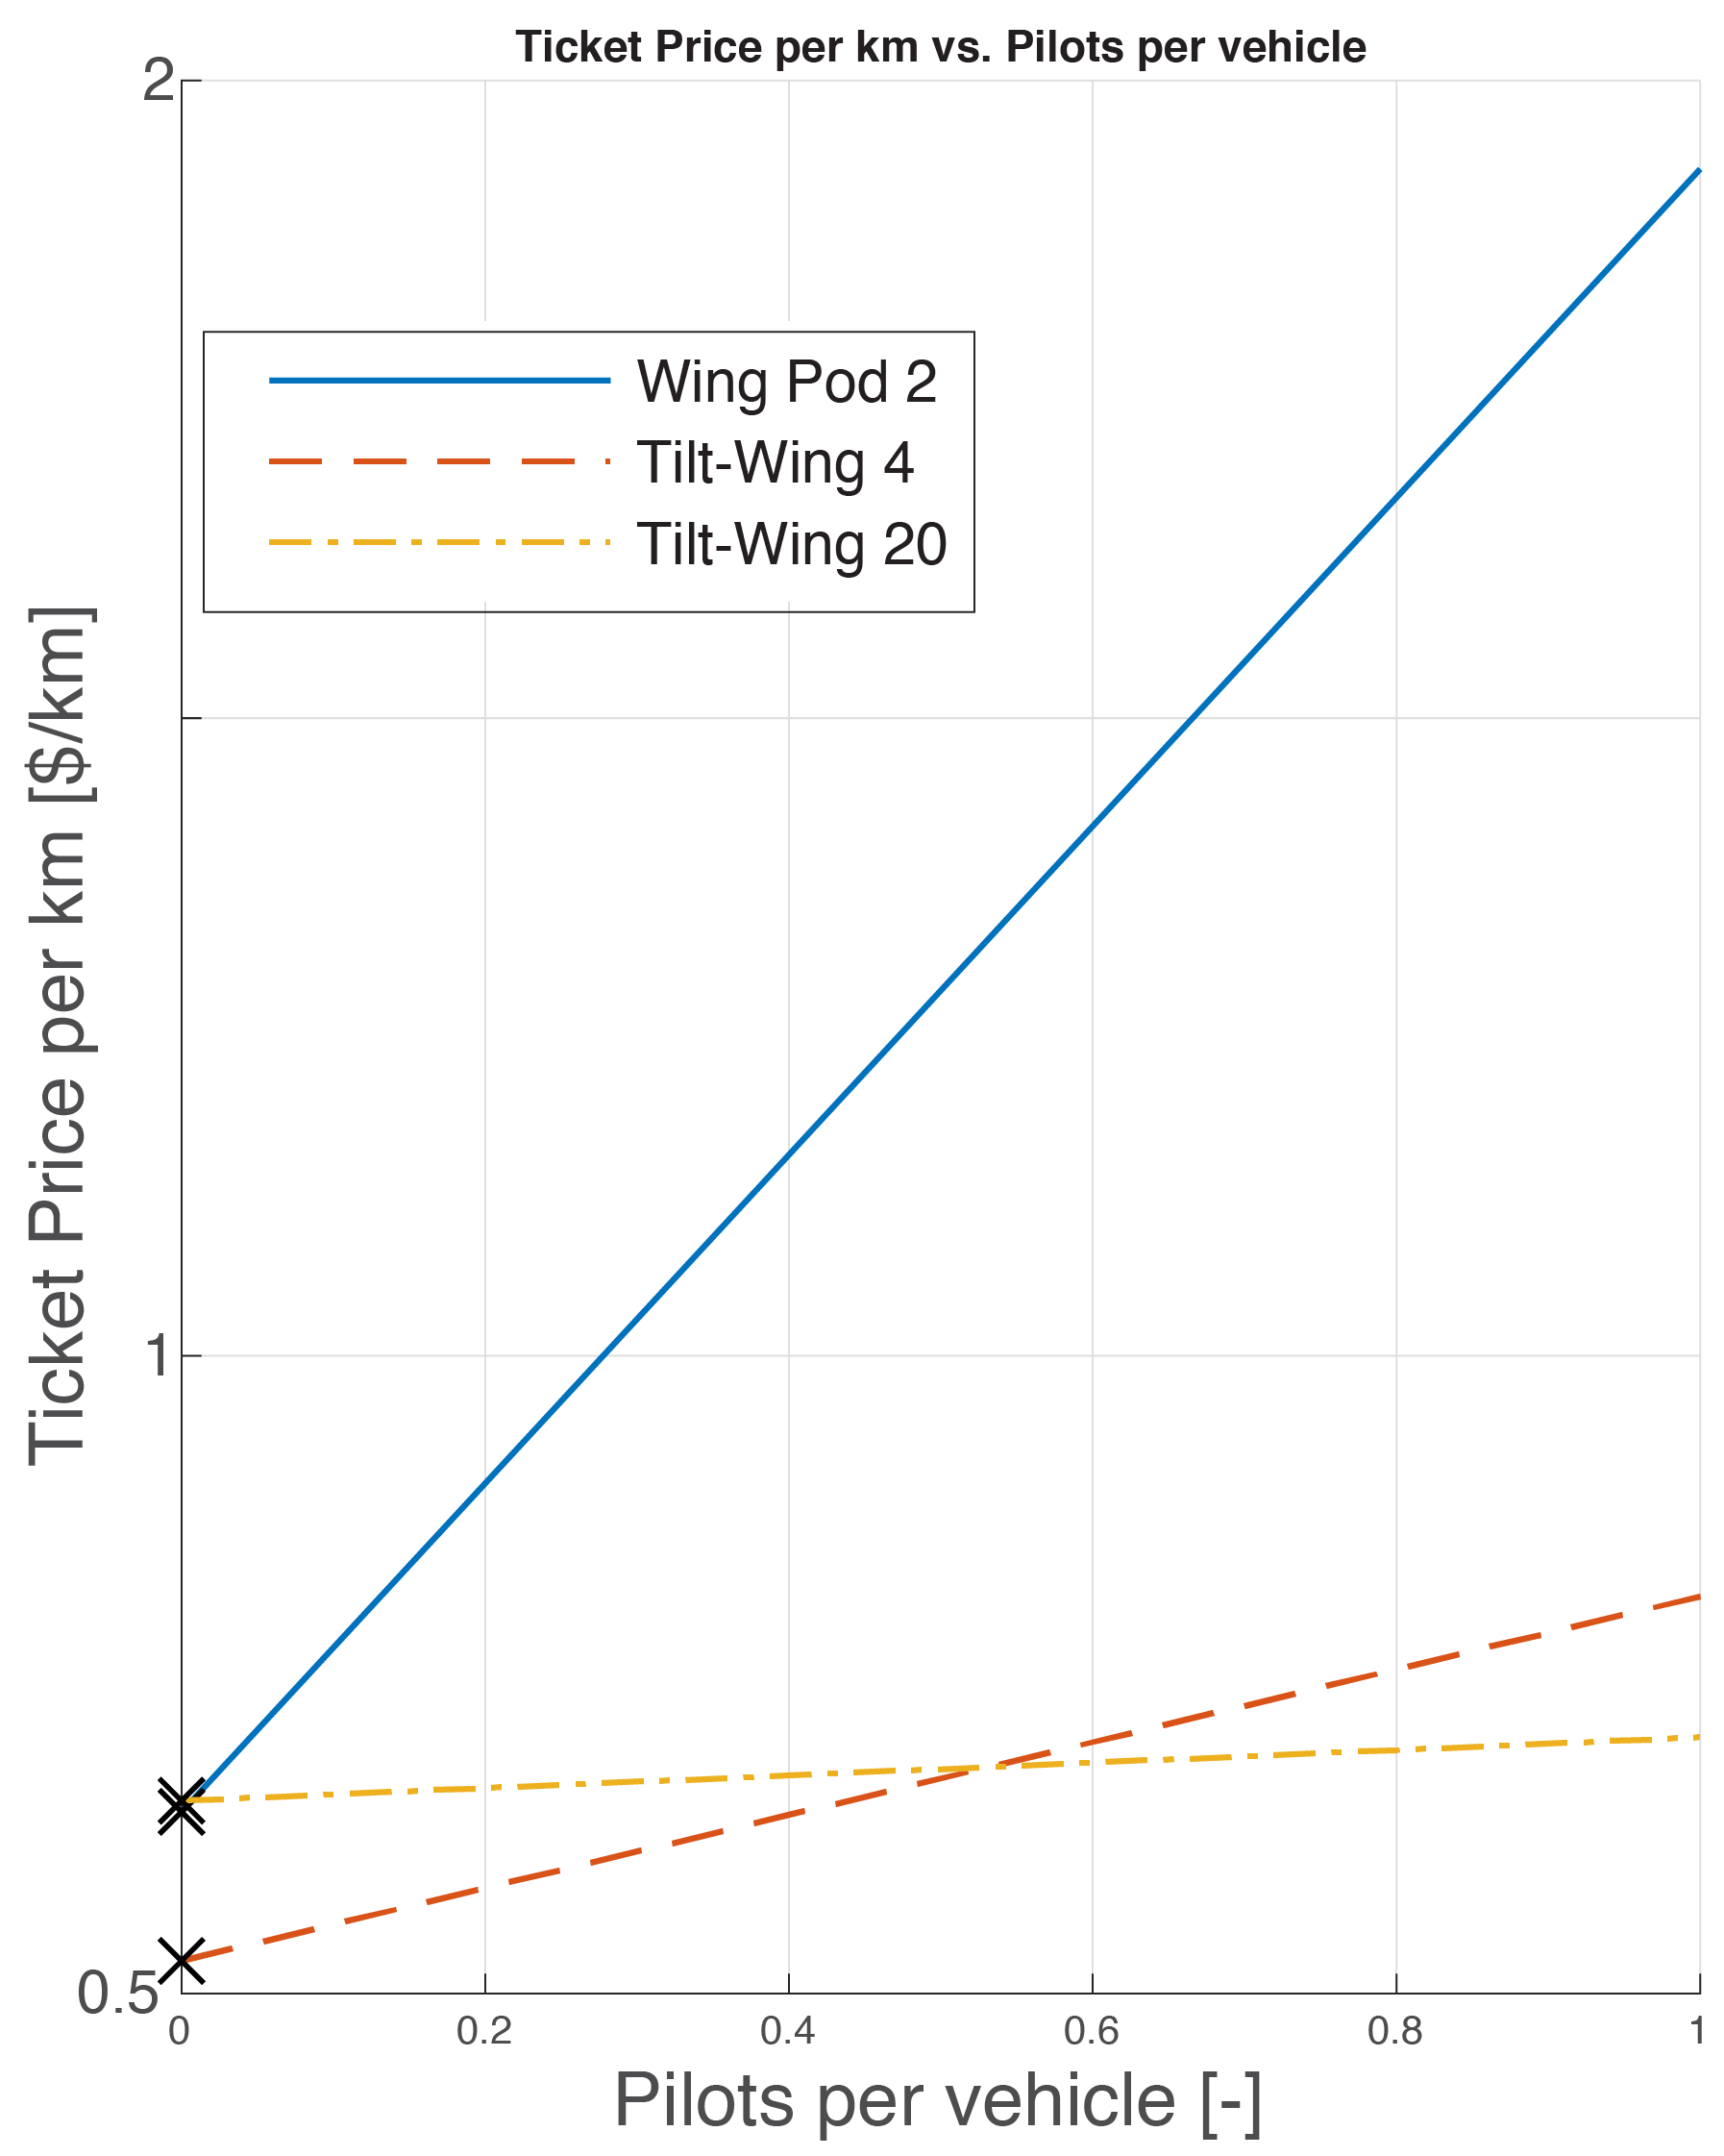
\includegraphics[width=0.35\textwidth]{Figures/autonomous_TPrice_perkm.png}
    \captionsetup{justification=centering}
    \caption{Ticket price increase due to including remote pilots, to assist autonomous vehicles.}
    \label{fig:autocost}
\end{wrapfigure}

Much of the trade-off has been done assuming that all the vehicles are completely autonomous. It is likely that remote piloting capabilities will be necessary for safety reasons. A pilot may need to intervene in certain situations. This also helps with a feeling of comfort for passengers. These pilots cost money, and will increase the operating cost per vehicle. By completing a sensitivity study based on the number of remote pilots, it can be shown at what point one concept may cost less than another. \autoref{fig:autocost} shows that the large vehicle benefits the most, and becomes cheaper (per km) to operate than the 4 passenger at 0.5 (1 pilot for every 2 vehicles). It seems more likely that less pilots will be required though.
